\section{Arduino}

O Arduino definido como uma plataforma eletrônica open-source baseada em hardware e software fáceis de usar. Sua simplicidade e flexibilidade tem permitido uma enormidade de projetos saírem do papel constantemente.

\subsection{Adicionar Bibliotecas do Arduino}

Com a revolução que o Arduino participa e promove, o uso de microcontroladores para diversos fins cresce exponencialmente. Seja automação residencial, devaneios de hobbystas ou robótica (móvel ou não), a versatilidade destes controladores é constantemente expandida. 

Com certos processos de maior complexidade pode ser interessante adicionar um protocolo, criado em .h e .c (ou .cpp), como biblioteca para o Arduino, pois um grande número de funções é comum para uma larga gama de projetos que a versatilidade do microcontrolador permite criar. Quando há um protocolo bem estabelecido como o de comunicação entre Arduino e PC, por exemplo, a adição do protocolo como biblioteca torna o desenvolvimento de aplicações mais simples, rápido e compreensível.

\subsubsection{Passos}

Os seguintes passos são necessários para a adição de bibliotecas:
\begin{enumerate}
\item Abrir a IDE do Arduino;
%Figura
\begin{figure}[!htb]
\centering
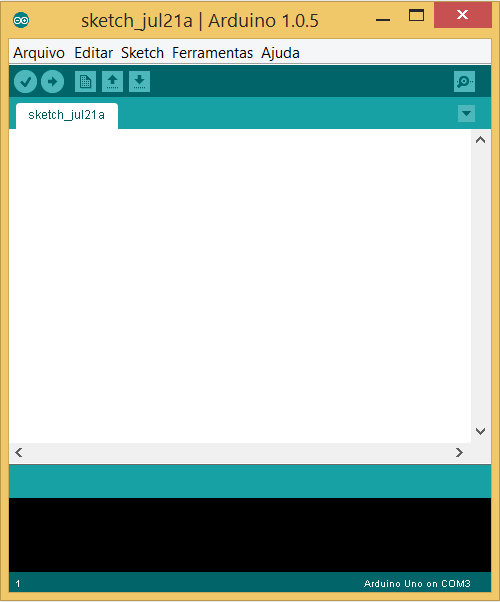
\includegraphics[width=3.7cm]{./include/chapters/sections/soft/section3/img/ide.png}
\caption{IDE Arduino}
\end{figure}
%Fim Figura
\item No Menu Sketch, selecione a opção Add Library;
%Figura
\begin{figure}[!htbp]
\centering
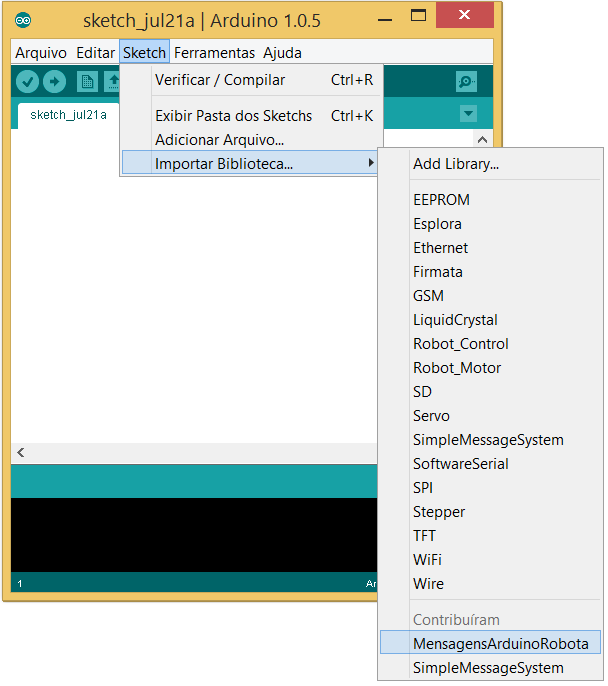
\includegraphics[width=4.5cm]{./include/chapters/sections/soft/section3/img/libadd.png}
\caption{Adicionar Biblioteca}
\end{figure}
%Fim Figura
\item Pronto. A biblioteca está adicionada. Agora é possível inclui-la no projeto com um simples include, como por exemplo 
\begin{lstlisting}
#include <MensagensArduinoRobota.h>
\end{lstlisting}
%Figura
\begin{figure}[!htbp]
\centering
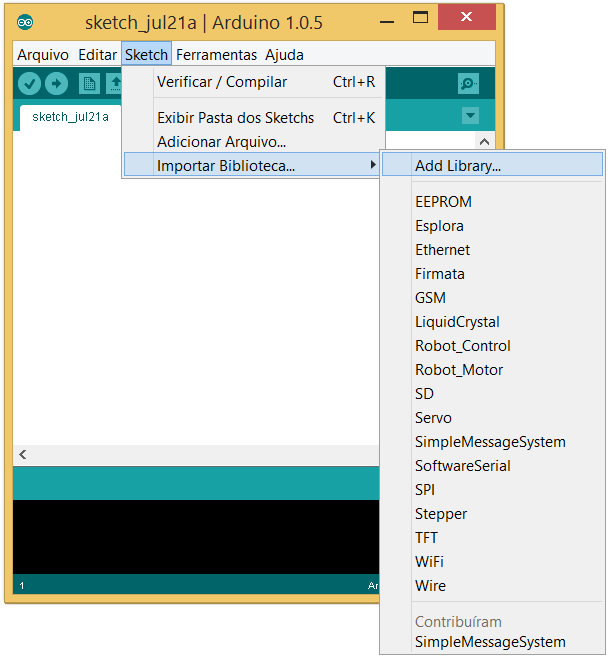
\includegraphics[width=4.5cm]{./include/chapters/sections/soft/section3/img/addlib.png}
\caption{Biblioteca adicionada}
\end{figure}
\end{enumerate}

Outra opção, um tanto menos sutil, é adicionar a pasta da biblioteca na pasta libraries no diretório onde o Arduino está instalado.

\subsection{Biblioteca MensagensArduinoRobota}

A Biblioteca "MensagensArduinoRobota" oferece aos usuários uma simples e intuitiva maneira de controlar um Arduino pelo computador.

\subsubsection{Funcionalidades}

As seguintes funcionalidades estão disponíveis:
\begin{itemize}
\item[•] Ler pinos digitais do Arduino;
\item[•] Ler pinos analógicos do Arduino;
\item[•] Chavear pinos digitais do Arduino;
\item[•] Escrever valores nos pinos de PWM do Arduino;
\end{itemize}

\subsubsection{Comandos}

Os comandos funcionam da seguinte forma:

O Arduino recebe uma string, pega a primeira letra de cada palavra para identificar o comando desejado e executa os comandos.

Os comandos resumem-se a:
\begin{itemize}
\item r $\to$ leitura
\item w $\to$ escrita
\item a $\to$ analógico
\item d $\to$ digital
\item t $\to$ todos
\item p $\to$ pino especifico para leitura
\end{itemize}

\subsubsection{Exemplos de comandos aceitos}

Alguns exemplos de comandos aceitos pela biblioteca:

\begin{itemize} 
\item r a t $\to$ Le todos os pinos Analogicos
\item r a p [pin] $\to$ Le valor do pino analogico especificado
\item r d t $\to$ Le todos os pinos digitais
\item r d p [pin] $\to$ Le valor do pino digital especificado
\item w d [pin] [value] $\to$ write digital pin
\item w a [pin] [value] $\to$ write analog pin
\end{itemize}

\subsubsection{Bibliografia}

Para a criação da presente biblioteca, os seguintes protocolos foram utilizados como exemplo:

\begin{itemize}
\item  Protocolo Firmata
\item  Protocolo CmdMessenger
\item  Protocolo SimpleMessagingSystem
\end{itemize}

\subsection{Visual C++ e Portas Seriais}

A utilização do Visual C++ para usos com o Arduino não é a maneira mais convencional encontrada, mas é uma possibilidade para alguns usuários. Existem diversas implicações negativas na escolha dessa linguagem de programação, mas existem alguns pontos positivos também. Apesar de não se ter a liberdade e praticidade que se tem ao trabalhar com periféricos via USB em S.O.s como o Ubuntu, o Visual C++ é uma alternativa funcional para utilizar C++, periféricos USB e o sistema Windows.

\subsubsection{Exemplo Visual C++ $\Rightarrow$ Porta Serial}

A seguir, exemplos simples do C++ no Windows para o controle de um Arduino conectado em uma porta USB de um PC.

O primeiro passo é adicionar uma biblioteca bastante importante para o uso de C++ e o Windows.
\begin{lstlisting}
// Biblioteca da malvada Microsoft para fazer tudo funcionar
#include "stdafx.h"
\end{lstlisting}

Com a biblioteca adicionada, é interessante definir os namespaces utilizados.
\begin{lstlisting}
using namespace System;
using namespace System::IO::Ports;
\end{lstlisting}

Agora, é possível definir a porta utilizada. No caso, a porta serial será chamada de Arduino para facilitar o processo.

\begin{lstlisting}
// Configuracao do Arduino
	int baudRate = 9600;
	portName = "COM3";
	SerialPort^ arduino;
	arduino = gcnew SerialPort(portName, baudRate)
\end{lstlisting}

É importante definir limites de tempo para a leitura e escrita de dados do Arduino.

\begin{lstlisting}
	arduino->ReadTimeout = 1500;
	arduino->WriteTimeout = 1500;
\end{lstlisting}

Para escrever algo na porta serial.

\begin{lstlisting}
	arduino->WriteLine("Algo");
\end{lstlisting}

Para ler algo da porta serial.

\begin{lstlisting}
	arduino->ReadLine();
\end{lstlisting}